\documentclass[12pt]{article}
\usepackage[spanish]{babel}
\usepackage{geometry}
\geometry{a4paper, margin=1in}
\usepackage{graphicx}
\usepackage{xcolor}
\usepackage{titlesec}
\usepackage{parskip}
\usepackage{multicol}
\usepackage{cite}
\usepackage{float}

\definecolor{highlight}{RGB}{255, 255, 0}

\titleformat{\section}{\normalfont\Large\bfseries}{\thesection}{1em}{}
\titleformat{\subsection}{\normalfont\large\bfseries}{\thesubsection}{1em}{}

\begin{document}

% Logos
\begin{minipage}{0.45\textwidth}
    
\includegraphics[width=0.4\textwidth]{inFiles/Figures/epnLogo.jpg}
\end{minipage}
\hfill
\begin{minipage}{0.45\textwidth}
    \raggedleft
    
\includegraphics[width=0.4\textwidth]{inFiles/Figures/FIS_logo.jpg}
\end{minipage}

\vspace{0.5cm}

% Títulos principales
\begin{center}
    \textbf{ESCUELA POLITÉCNICA NACIONAL}\\[0.2cm]
    \textbf{FACULTAD DE INGENIERÍA DE SISTEMAS}\\[0.2cm]
    \textbf{INGENIERÍA {\textbf{EN COMPUTACIÓN}}}
\end{center}

\vspace{0.5cm}
\hrule
\vspace{0.5cm}

% Datos principales
\noindent\textbf{PERÍODO ACADÉMICO:} 2025-A\\[0.2cm]
\noindent\textbf{ASIGNATURA:} ICCD412 Métodos Numéricos \hfill \textbf{GRUPO:} GR2\\[0.2cm]
\noindent\textbf{TIPO DE INSTRUMENTO:} Tarea 1\\[0.2cm]
\noindent\textbf{FECHA DE ENTREGA LÍMITE:} 04/05/2025\\[0.2cm]
\noindent\textbf{ALUMNO:} Murillo Tobar Juan

\vspace{0.5cm}
\hrule
\vspace{1cm}


% Secciones
\section*{TEMA}
Tipos de errores
\vspace{0.5cm}

\section*{OBJETIVOS}
\begin{itemize}
    \item Conocer los límites de nuestros sistemas para evitar errores en la codificación de programas relacionados con la materia de métodos numéricos. 
    \item Reproducir desbordamientos de memoria para el futuro reconocimiento y manejo de estos posibles errores. 
\end{itemize}

\vspace{0.5cm}

\section*{MARCO TEÓRICO}
\colorbox{highlight}{No solicitado} 

\vspace{0.5cm}

\section*{DESARROLLO}
Para esta tarea se requería de identificar los límites de datos en nuestros computadores y ver que sucede al desbordar esos límites en PYTHON. 
Para la primera parte utilizamos la librería sys como se puede ver en la siguiente captura.


\begin{figure}[H]
\centering
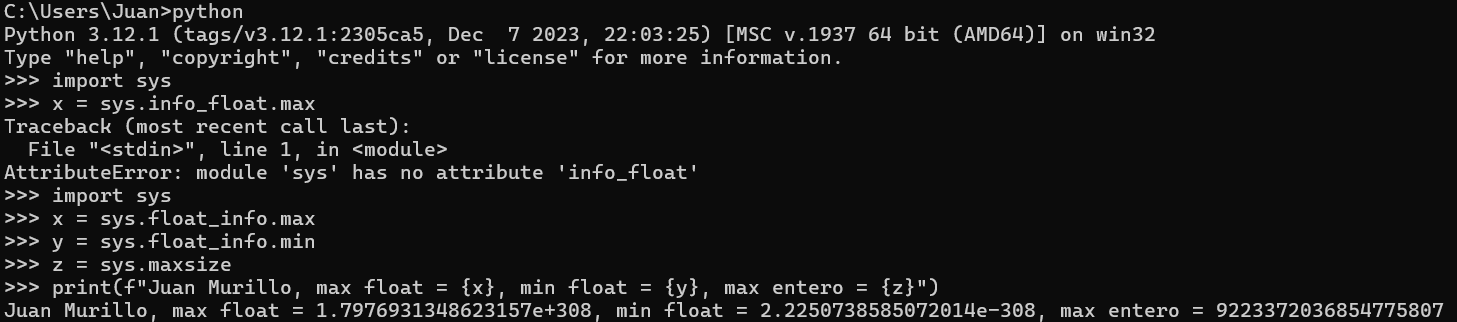
\includegraphics[width=1\textwidth]{./inFiles/Figures/Cap1.png}
\caption{Captura de Python}
\end{figure}

En la segunda parte debíamos desbordar dichos valores para obtener nan en los resultados.
\begin{figure}[H]
\centering
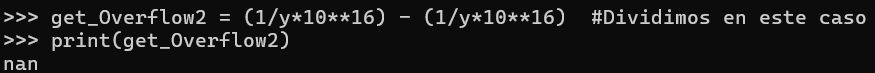
\includegraphics[width=1\textwidth]{./inFiles/Figures/Cap2.png}
\caption{Desbordamiento del valor float max positivo}
\end{figure}

\begin{figure}[H]
\centering
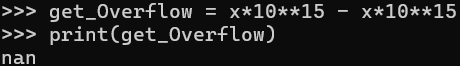
\includegraphics[width=1\textwidth]{./inFiles/Figures/Cap3.png}
\caption{Desbordamiento del valor float min positivo}
\end{figure}

En el caso de los enteros surge un inconveniente. Como se menciona en \cite{python}, en enteros no puede darse el caso de Overflow, por lo que en este caso unicamente buscamos un MemoryError que en algunos sistemas es el congelamiento de la terminal.
\begin{figure}[H]
\centering
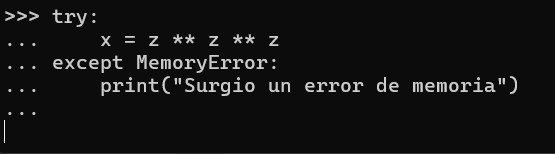
\includegraphics[width=1\textwidth]{./inFiles/Figures/Cap4.png}
\caption{Congelamiento de la terminal}
\end{figure}

\vspace{0.5cm}


\vspace{0.5cm}


\renewcommand{\refname}{\MakeUppercase{REFERENCIAS}}
\bibliographystyle{IEEEtran}
\bibliography{inFiles/References/references.bib}

\end{document}
